\section{データセット}
本節では,本研究で用いるデータセットについて紹介する.

\subsection{本調査の対象}
次の条件を満たすリポジトリを対象とした.
\begin{itemize}
    \item スターが10個以上あること
    \item 最終更新が2021年以降であること
    \item issueが一つ以上あること
\end{itemize}
スター数の条件は,本研究に関連する可能性が低いプロジェクト(個人のプロジェクトやサンプルプロジェクトなど,不具合報告が発生しにくいもの)
を除外するために設定した.
また,最終更新を2021年以降に限定することで,より近年の動向を得られると判断した.
すべての条件を満たすリポジトリは,289,115件であった.
これらのリポジトリから4,173件のリポジトリをランダムに選んだ.
4,173件のリポジトリから,770,656件の解決済みのIssueを取得した.
データ収集期間は2021年11月から12月であり,件数は当時のものである.

\subsection{データ取得内容と方法}
本調査で用いるIssueの8つの調査項目を紹介する.調査項目を表~\ref{issue_parameter}に示す.

\begin{table}[t]
    \begin{center}
    \caption{issueの調査項目}
    \renewcommand{\arraystretch}{1.3}
    \begin{tabular}{l|l} 
        \hline
        調査項目 & 内容 \\ 
        \hline \hline
        $Issue\_open\_time$ & Issueが解決するまでの時間(日) \\
        $First\_comment\_time$ & 最初のコメントがつくまでの時間(日) \\
        $Num\_of\_comments$ & 寄せられたコメント数 \\
        $Num\_of\_char$ & Issueの作成時の文字記述量 \\
        $Num\_of\_img$ & Issueの作成時の画像添付数 \\
        $Num\_of\_mov$ & Issueの作成時の動画添付数 \\
        $Words$ & Issueの作成時の記述された英単語 \\
        $Issue\_created\_at\_year$ & Issueが作成された年 \\
        \hline
    \end{tabular}
    \label{issue_parameter}
    \end{center}
\end{table}

Issueの調査項目は,GitHub~APIであるPyGithub(pythonライブラリ)を用いて取得した.
$Num\_of\_char$,$Num\_of\_img$,$Num\_of\_mov$,$Words$は直接取得できないため,その取得方法を紹介する.
Issueに貼り付けた動画及び画像はURLに変換され,Issueのテキスト(直接取得可能)にマークダウン形式で記述される.
URLに変換された一例を次に示す.\\

https://user-images.githubusercontent.com/XXX.mp4 \\

XXXの部分は,半角英数字,"/","-"のみで構成される.

従って,以上のURLを正規表現で取得し出現回数を,拡張子に応じて$Num\_of\_img$,及び,$Num\_of\_mov$とした.\\

動画及び画像を含むIssueについて,上記URLを除外処理したテキストを用いて,$Words$を正規表現で取得した.
また,処理済みのIssueのテキストの長さを,$Num\_of\_char$とした.


我々は事前調査で,$Issue\_open\_time$が,何らかの要因により負値をとるIssueが混在していることを発見した.
このような不正な値を含むIssueを除外するため,30seconds <= $Issue\_open\_time$ <= 1yearの条件を設けた.
この条件を満たすIssueは,711,160件(92.23\%)であった.


\subsection{データの分類}
動画及び画像の有無でIssueを次の3つのカテゴリに分類した.\\

\begin{tabular}{c l}
    $Img$ & $Num\_of\_img$が1以上のIssue \\
    $Mov$ & $Num\_of\_mov$が1以上のIssue \\
    $None$ & 上記どちらにも含まれないIssue\\ 
\end{tabular} \\

ただし,動画と画像をどちらも含むIssueは$Img$及び$Mov$の両方に属す.
各Issue群の要素数を表\ref{classify_result}に示す. 

\begin{table}[h]
    \begin{center}
    \caption{カテゴリー分類・要素数}
    \begin{tabular}{c|c|c}
        \hline
        $Img$ & $Mov$ & $None$ \\ 
        \hline \hline
        33,079 (4.65\%) & 3,819 (0.54\%) & 674,793 (94.81\%) \\
        \hline
    \end{tabular}
    \label{classify_result}
    \end{center}
\end{table}


収集したデータの一部抜粋を表\ref{dataset_example}に示す.
1つのIssueの情報が表の行に並んでおり,$Issue\_open\_time$及び$First\_comment\_time$の単位は日数である.

\begin{table*}[h]
    \begin{center}
    \caption{取得したIssueの調査項目の一部抜粋}
    \begin{tabular}{c c c c c c c} 
      \hline
      \begin{tabular}{c} \textbf{Issue\_created}\\\textbf{\_at\_year} \end{tabular} &
      \begin{tabular}{c} \textbf{Issue\_open}\\\textbf{\_time} \end{tabular} &
      \begin{tabular}{c} \textbf{Num\_of}\\\textbf{\_img} \end{tabular} &
      \begin{tabular}{c} \textbf{Num\_of}\\\textbf{\_mov} \end{tabular} &
      \begin{tabular}{c} \textbf{Num\_of}\\\textbf{\_comments} \end{tabular} &
      \begin{tabular}{c} \textbf{First\_comment}\\\textbf{\_time} \end{tabular} &
      \begin{tabular}{c} \textbf{Num\_of}\\\textbf{\_char} \end{tabular} \\
      \hline \hline
      2020 & 6.99861111 & 0 & 0 & 1 & 6.99861111 & 39488\\
      2020 & 41.9594329 & 1 & 0 & 3 & 17.7784722 & 950\\
      2020 & 43.8850579 & 0 & 0 & 2 & 0.49828704 & 379\\
      2020 & 44.0935532 & 0 & 0 & 4 & 0.91277778 & 191\\
      2020 & 0.14934028 & 0 & 0 & 8 & 0.08077546 & 1800\\
      2020 & 59.5670949 & 2 & 0 & 5 & 0.39472222 & 999\\
      2020 & 74.9322569 & 0 & 0 & 0 & -          & 127\\
      \hline
    \end{tabular}
    \label{dataset_example}
    \end{center}
  \end{table*}

%\begin{figure*}[t]
%    \begin{center}
%        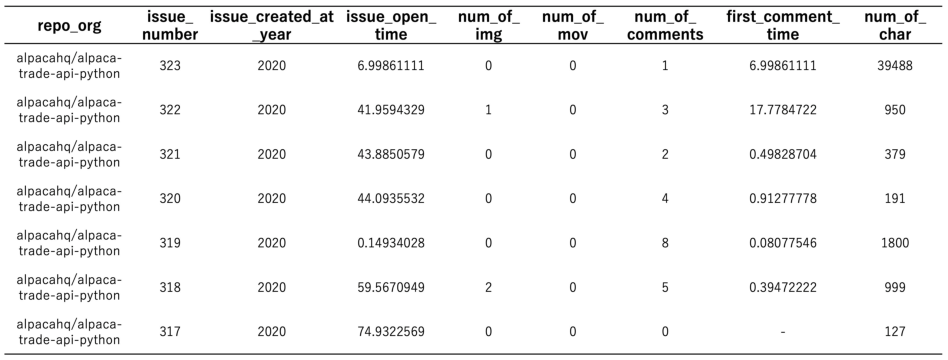
\includegraphics[scale=1.1]{./image/dataset_example.pdf}
%        \caption{取得したIssueの調査項目の一部抜粋 \label{dataset_example2}}
%    \end{center}
%\end{figure*}
